	
	\documentclass[12pt,journal,compsoc]{IEEEtran}
	\usepackage[utf8]{inputenc}

	% *** CITATION PACKAGES ***
	\usepackage[nocompress]{cite}
	%\usepackage{cite}

	% *** GRAPHICS RELATED PACKAGES ***
	\usepackage[pdftex]{graphicx}
	\usepackage{framed}
	\graphicspath{{img/}}
	\DeclareGraphicsExtensions{.pdf,.jpeg,.jpg,.png}

	% *** MATH PACKAGES ***
	\usepackage[cmex10]{amsmath}

	% *** SPECIALIZED LIST PACKAGES ***
	\usepackage[footnote]{acronym}
	\usepackage{algorithm2e}
	\usepackage{alltt}

	% *** ALIGNMENT PACKAGES ***
	\usepackage{array}
	\usepackage{mdwmath}
	\usepackage{mdwtab}
	\usepackage{eqparbox}

	% *** SUB FIGURE PACKAGES ***
	\usepackage[caption=false,font=normalsize,labelfont=sf,textfont=sf]{subfig}
	%\usepackage[caption=false,font=footnotesize]{subfig}

	% *** FLOAT PACKAGES ***
	\usepackage{dblfloatfix}

	% *** PDF, URL AND HYPERLINK PACKAGES ***
	\usepackage{url}
	
	% *** COLORS ***
	\usepackage[usenames,dvipsnames]{color}

	\newcommand\MYhyperrefoptions{bookmarks=true,bookmarksnumbered=true,
	pdfpagemode={UseOutlines},plainpages=false,pdfpagelabels=true,
	colorlinks=true,linkcolor={black},citecolor={black},urlcolor={black},
	pdftitle={Efficient 3D Isotropic Volume Reconstruction Based On 2D Localized Ultrasound Images},
	pdfsubject={Introduction To Lab Research},
	pdfauthor={Keck Jean-Baptiste},
	pdfkeywords={Introduction to Lab Research, Arthrosis, GPGPU, Ultrasound Imaging, Isotropic Volume Reconstruction}}

        \acrodef{gpgpu}[GPGPU]{General Purpose Computing on Graphics Processing Unit}
        \acrodef{cuda}[\texttt{CUDA}]{Compute Unified Device Architecture}
        \acrodef{timcimag}[TIMC-IMAG]{Techniques de l’Ingénierie Médicale et de la Complexité - Informatique, Mathématiques et Applications, Grenoble}
        \acrodef{gmcao}[GMCAO]{Gestes Médico-Chirurgicaux Assistés par Ordinateur}
	\acrodef{ssd}[SSD]{Solid-State Drive}
	\acrodef{hdd}[HDD]{Hard Disk Drive}
	\acrodef{simd}[SIMD]{Single Instruction, Multiple Data}
	\acrodef{vnn}[VNN]{Voxel Nearest Neightbor}
	\acrodef{pnn}[PNN]{Pixel Nearest Neightbor}
	\acrodef{dw}[DW]{Distance Weighted}

	\begin{document}

	\title{Efficient 3D Isotropic Volume Reconstruction Based On 2D Localized Ultrasound Images}

	\author{Jean-Baptiste~Keck,~\IEEEmembership{Student,~Ensimag}
		Matthieu~Chabanas,~\IEEEmembership{Supervisor,~TIMC-IMAG Laboratory}%
	\IEEEcompsocitemizethanks{%
	\IEEEcompsocthanksitem M. ~Keck is a student at Ensimag, Grenoble, France.
	\IEEEcompsocthanksitem M. ~Chabanas is in the team Gestes Médico-Chirurgicaux Assistés par Ordinateur in the TIMC-IMAG Laboratory, University of Grenoble, France.}}

	\markboth{Introduction to Laboratory Research, Report,~Version.~2, May~2014}%
	{shell test}

	\IEEEspecialpapernotice{TIMC-IMAG}

	\IEEEtitleabstractindextext{%
	\begin{abstract}
		A miniature 3D tracked ultrasonic probe has been developed to acquire intra-articular cartilage images under arthroscopic surgical conditions. The aim is to detect cartilaginous lesions (arthritis) and quantify their precise sizes and locations to help the clinician in his diagnostic and his therapeutic decision making.
		The ultrasonic transducer is tracked by an optical sensor, which permits to find location and orientation of each 2D US images in a common 3D spacial reference. Near two thousands images are acquired when scanning a cartilage surface. An interesting tool is to rebuild a 3D isotropic volume (cubic voxels) with those images, allowing further processing.
		Conventional 3D ultrasound algorithms have low computational complexity but the huge amount of data generated makes it difficult to compute results within reasonable time on classical computers. In this paper we investigate the possibilities of regenerating a 3D isotropic volume with the help of \ac{gpgpu} (CUDA) by adapting existing algorithms to massive parallelism provided by modern everyday GPUs.
	\end{abstract}

	\begin{IEEEkeywords}
		Introduction to Lab Research, Arthritis, \acl{gpgpu}, Ultrasound Imaging, Isotropic Volume Reconstruction.
	\end{IEEEkeywords}%
	}	
	
	\maketitle


% make the title area

\section{Introduction}

\IEEEPARstart{F}{reehand} three-dimensional ultrasound imaging is a highly attractive research area because it is capable of volumetric visualization and analysis of tissue and organs. Conventional two-dimensional ultrasound imaging has been widely used for many clinical applications such as medical diagnosis and image-guided surgery. In comparison with Computed Tomography (CT) and Magnetic Resonance Imaging (MRI), ultrasound imaging is non invasive, real time, portable and low cost. However, 2D ultrasound imaging fails to offer clinicians whole volume data for visualization and analysis. Thus three-dimensional ultrasound imaging systems has been developed to overcome those limitations by constructing various 3D datasets. Several approaches for constructing 3D ultrasound volume data have been reported. These approaches can be classified into three categories : dedicated 3D probes, mechanical scanning approach, and freehand scanning approach. 
Dedicated 3D probes can provide 3D data in real time but they are expensive and have limitations in scanning large volume organs.
The mechanical scanning approaches usually use conventional 2D transducers which are translated and rotated with stepping motors. This design creates limitations in term of their scanning range. 
Finally, freehand ultrasound use conventional 2D transducers in pair with a positioning sensor to save position and orientation of each acquired image.
Freehand 3D ultrasound has received increasing attention for it's low cost and flexibility, as it allows the user to manipulate and view the desired anatomical section freely.

Cartilage diseases represent a major Public Health problem that will worsen due to the ageing of the population and the obesity epidemic.
The development of new diagnostic and therapeutic strategies therefore appears to be essential to address this issue.
The research project “Computer Assisted Measures and Interventions for Innovative Therapeutic of Cartilage Diseases” led to the development of a new medical device dedicated to the therapy of the cartilaginous tissue: a navigated multimodal arthroscopic environment.
It combines MRI or arthro-CT with video and ultrasound. 
A special probe was specially designed to acquire intra-articular cartilage images under arthroscopic surgical conditions with the aim of reconstructing the cartilage surface.

During scanning a sequence of US images are captured along with their positions and orientations, synchronously. Those data are then used to reconstruct a 3D volume by using various interpolation or approximation algorithms. The reconstruction algorithm plays a key role in the construction of three-dimensional ultrasound volume data with higher image quality and faster reconstruction speed.\par

Even if conventional 3D reconstruction algorithms have low computational complexity, the huge amount of data generated by a single scan (thousands of 2D images) makes it difficult to compute volume data in reasonable clinical time on classical computers.
This paper aims to speed up 3D volume processing by adapting existing reconstruction algorithms to the massive parallelism provided by nowadays affordable GPUs. This is achieved through \acl{gpgpu} (\ac{gpgpu}), a concept that has been well developed and widely adopted during the last decade and that continues its growth.
The Open Computing Language (OpenCL) is the currently dominant open general-purpose GPU computing language. The dominant proprietary framework is the \acl{cuda} (CUDA).
Although \texttt{cuda} requires a Nvidia \texttt{CUDA} compatible graphic card, we choose it because of its more mature status (performance and debugging tools) but algorithms are easily adaptable to OpenCL as well, allowing executions on Nvidia's and AMD's graphic cards, and even Integrated Graphics Processors (IGPs).


\section{System overview}

\begin{figure}[!ht]
\centering
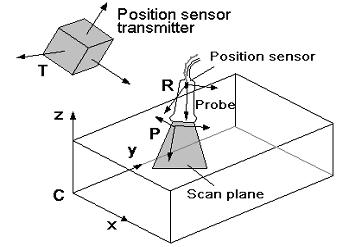
\includegraphics[width=2.5in]{freehand}
\caption{A classical freehand ultrasound imaging system setup. Image taken from T. Wen \textit{et al.}\cite{2}.}
\label{fig_1}
\end{figure}


\subsection{System setup}

The freehand 3D ultrasound imaging system consists of three modules : a 2D ultrasound scanner specially designed to acquire intra-articular cartilage US images under arthroscopic surgical conditions, an optical position and orientation sensor and a work station with custom designed software for data acquisition. The volume reconstruction is for the moment done as a post-process in another specially designed piece of software.
The portable ultrasound scanner consists of 64 axis-aligned transducers. Although it is a freehand system, the axe is slightly rotated by a stepper motor to achieve a greater scanning area. The transformation due to the rotation of the motor is taken in account.

\begin{figure}[hb!]
\centering
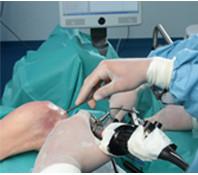
\includegraphics[width=2.5in]{miticao}
\caption{The freehand ultrasound system acquiring intra-articular cartilage images under arthroscopic surgery conditions.}
\label{system1}
\end{figure}


The receiver of the spacial sensing device is attached to the hand-held probe of the ultrasound scanner. Another receiver is attached to the head of the femur. This allow us to record the position and orientation of the scanned US images with regard to the femur. 
During data acquisition, spacial data and digitalized 2D scans are simultaneously recorded and collected. Images which attack rate is too high are discarded as there is too much distorsion in the ultrasound signal that is sent back to the probe. \textbf{Fig.\ref{system1}} and \textbf{fig.\ref{system2}} show the probe in action and a more detailed schematic of the system.
%Since the ultrasound probe and the spacial sensor are independent, the temporal delay between two data streams can not be avoided. 


\begin{figure}[ht!]
\centering
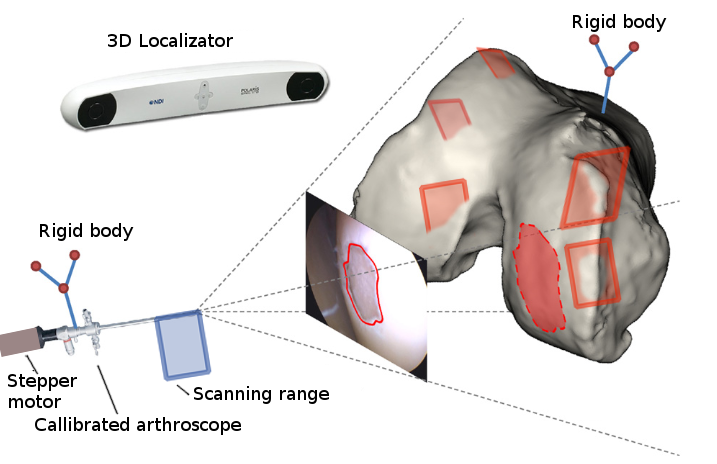
\includegraphics[width=3.5in]{system}
\caption{The freehand ultrasound imaging system setup, including the optical position sensor, two rigid bodies (reflectors), the motorized freehand arthroscope and the scanning range of the 64 transducers. The two scans on the right are discarded.}
\label{system2}
\end{figure}


\subsection{Data acquisition}

After signal processing 2D slices of logical size $L_x$ x $L_y = 64\times 1296$ pixels are generated. 
As the transducers are $\epsilon_x=205\mu m$ wide, the images have a physical size of $P_x = 64\;\epsilon_x=19.12mm$. 
The precision on the other axe is $\epsilon_y=18\mu m$, and thus the images have a physical height of $P_y = 1296\;\epsilon_y=23.328mm$.
For the images we will use this convention : we place the origin at the top-left with the x-axis oriented towards the right and the y-axis oriented towards the bottom. 
We define $X_p=(x_p,y_p,0,1)^T$ the homogeneous vector that describes logical position of each pixel $(x_p,y_p)$ in an image whose origin is at $(O_x,O_y)$. 
$S_x$ and $S_y$ are the pixel spacing on each axis and are defined as $S_x = \frac{P_x}{L_x}$ and $S_y = \frac{P_y}{L_y}$. 

\begin{equation}
	M_{model} = \left(
	\begin{IEEEeqnarraybox*}[][c]{,c/c/c/c,}
		$$
		S_x&0&0&O_x\\
		0&S_y&0&O_y\\
		0&0&0&0\\
		0&0&0&1%
		$$
	\end{IEEEeqnarraybox*}
\right)
\end{equation}

\begin{samepage}
The physical position of each pixel in its local physical coordinate system can be calculated as the following : 
\begin{IEEEeqnarray}{rCl}
X_m = M_{model}\;X_p
\end{IEEEeqnarray}
\end{samepage}

$M_{RP}$ is the transformation matrix from the optical position sensor reflector (R) to origin of the scanned image plane (P), $M_{ER}$ is the transformation matrix from the optical emitter (E) to (R) and $M_{VE}$ is the transformation matrix from the voxel coordinate of the reconstructed volume (V) to (E). Note that all those matrices are 4x4 homogeneous matrices.

$M_{RP}$ is initially unknown and must be obtained through a calibration process. For a detailed discussion for this issue, one can refer to Mercier \textit{et al.}\cite{8}.

With those matrices and (1), the whole forward transformation can be written as : 

\begin{IEEEeqnarray}{rCl}
X_v = M_{VE}M_{ER}M_{RP}\;X_m = M\;M_{model}\;X_p
\end{IEEEeqnarray}

The specially designed software used to acquire data can export each image in a MHD file format (MetaImage Format in ITK). Mhd files contain header informations, including transformation matrix M and size, and raw image data.

\begin{figure}[!hb]
\centering
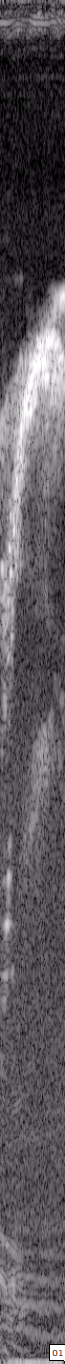
\includegraphics[width=40mm, height=50mm]{scan}
\caption{A typical 2D ultrasound image of intra articular cartilage. The white band is the cartilage interface.}
\label{fig_2}
\end{figure}


\begin{figure}[ht!]
\centering
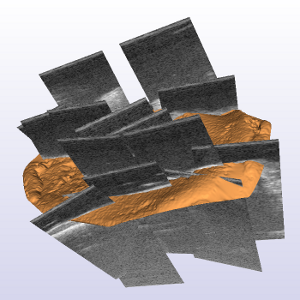
\includegraphics[width=2.5in]{us_images}
\caption{Scanned US images after transformation (3). Here the cartilage interface was reconstructed from MRI data.}
\label{system}
\end{figure}


\section{Volume Reconstruction}

\subsection{Reconstruction steps}

%After the 2D images and positions are exported as raw and mhd files, the next procedure is to reconstruct a 3D volume data. 
Here is were my work began.
Given the sampled images from first step \{$I_i$\} and the transformation matrices \{$M_i$\}, the aim was to reconstruct 3D volume data.

\vspace{0.5cm}
Here is the flow diagram of freehand 3D ultrasound volume reconstruction :
\vspace{0.5cm}
\begin{framed}
\noindent\textbf{Step 1 : Data loading}
\begin{itemize}
	\item Parse mhd files
	\item Load image raw data
	\item Load transformations
\end{itemize}
\textbf{Step 2 : Data preprocessing}
\begin{itemize}
	\item Position filtering
	\item Image filtering
	\item Image cropping
	\item Image data conversion
\end{itemize}
\textbf{Step 3 : Grid construction}
\begin{itemize}
	\item Determinate grid size
\end{itemize}
\textbf{Step 4 : Volume Filling}
\begin{itemize}
	\item Bin-filling
	\item Hole-filling
\end{itemize}
\end{framed}

\newpage
\subsection{Data loading}

Loading data is not as easy as one might think and can rapidly become a serious bottleneck compared to what GPGPU can provide in terms of speedup. 
As each US scan is exported in its own mhd and raw file, thousands of mhd files have to be parsed to get each transformation matrix \{$M_i$\} and get the path to the corresponding image data and load the raw image \{$I_i$\}.  
With two thousands images this operation can easily take 2 minutes on regular \ac{hdd} and even half a minute on a \ac{ssd}.
One easy fix would be to merge all the image data into a single raw file, and the transformation matrices in another raw file as well, or simply keep the generated data in the computer memory when doing on the fly or immediate post-processing.
Data locality is something we do not only want on the disk, but in the memory too. This introduces an important concept : Array of Structures (AoS) versus Structure of Arrays (SoA). In GPGPU, memory access are a serious bottleneck when done improperly and SoA are often the better solution than AoS. 

For example, a list of 3D vectors can be represented with 3 arrays, one for each of its coordinates (SoA), or with an array of 3D vector structures (AoS) :

\begin{samepage}
\begin{alltt}
\textbf{Structure of Arrays (SoA):}
struct vectors \{
    float x[100];
    float y[100];
    float z[100];
\}

struct vectors v;

\textbf{Array of Structures (AoS):}
struct vector \{
    float x;
    float y;
    float z;
\}

struct vector v[100]
\end{alltt}
\end{samepage}

\newpage
When using a structure of arrays we have memory spacial locality between each of the vector coordinates. When a memory read occur in the global memory of a GPU, a large chunk of data is read (most of the time 256 bytes memory segments aligned on 256-byte address). This is because the GPU is a massive parallel architecture.
In \texttt{CUDA}, threads are grouped into thread blocks, which are assigned to multiprocessors on the device. During execution there is a finer grouping of threads into warps. Multiprocessors on the GPU execute instructions for each warp in \acl{simd} fashion. The warp size of current \texttt{CUDA}-capable GPUs is 32 threads. 
The device coalesces global memory loads and stores issued by threads of a warp into as few transactions as possible to minimize memory bandwidth.
Any misaligned access by a half warp of threads results in 16 separate 32-byte transactions. If only 4 bytes are requested per 32-byte transaction (a simple integer or float), we should expect the effective bandwidth to be reduced by a factor of eight.
For strided global memory access things get even worse, and get worser when the stride get bigger.
That is not surprising because when concurrent threads simultaneously access memory addresses that are very far apart in physical memory, then there is no chance for the hardware to combine the accesses.
Strides entailed by Array of Structures is the reason why we want to use Structure of Arrays, where data is nicely arranged to be accessed in a parallel manner.

Taking this into account, we decompose the 4x4 homogeneous transformation matrices \{$M_i$\} into a structure of 12 arrays, the 3x3 inner rotation matrix coefficients $r^1$ through $r^9$, and the 3D offset vector coefficients $(x,y,z)$ :

\begin{equation}
	M_i = \left(
	\begin{IEEEeqnarraybox*}[][c]{,c/c/c/c,}
		$$
		r_i^1&r_i^2&r_i^3&x_i\\
		r_i^4&r_i^3&r_i^5&y_i\\
		r_i^5&r_i^6&r_i^7&z_i\\
		0&0&0&1%
		$$
	\end{IEEEeqnarraybox*}
\right)
\end{equation}

The matrix is initially stored in a row-major manner, this is why we use such indexing convention for $r_i$.

\begin{samepage}
\begin{alltt}
\textbf{The resulting struct is :}
struct transformations \{
    //offsets
    float *x;
    float *y;
    float *z;

    //3x3 matrix coefficients
    float *r1;
    float *r2;
    ...
    float *r9;
\}

\end{alltt}
\end{samepage}

\begin{figure*}[!ht]
\centering
\subfloat[Original image]{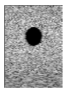
\includegraphics[width=1.0in, height=1.5in]{image_filtering_orig}%
\label{image_filtering_orig}}
\hfil
\subfloat[Filtered image]{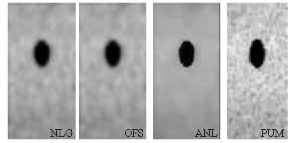
\includegraphics[width=3in]{image_filtering_comp}%
\label{fig_second_case}}
\caption{An example of ultrasound image smoothing techniques taken from A. Babakhani \textit{et al.}\cite{1}}
\label{comparisson_smoothing}
\end{figure*}

Image data do not require such memory reorganization as it is already stored and loaded as a row-major matrix of black and white pixels represented by simple precision floats. We just pay a special care to load the images in a big contiguous memory space and not to load them at random locations into the memory.
Of course if the images were color images, we would have separated the red, green and blue channels into three separate arrays in a SoA manner. \par

This is not the only thing to take into account when loading data into memory when using GPGPU.
When allocating CPU memory (RAM) that will be used to transfer data to the GPU memory (VRAM) for computing purpose, there are two types of memory to choose from : pinned (page-locked) and non-pinned memory. 
Pinned memory is memory specially allocated with a GPGPU dedicated malloc function (cudaMallocHost in \texttt{CUDA}), which prevents the memory from being swapped out and provides improved transfer speeds. 
Non-pinned memory is memory allocated using the classical malloc function in C, or using the new operator in \texttt{C++}. 
Pinned memory is much more expensive to allocate and deallocate but provides higher transfer throughput for large memory transfers.
Empirically, using pinned memory only makes sense when the amount of memory transferred each way is larger than 16 MB. 
In our case with 2000 US scans, we have 664MB of float images, and 96Ko of transformations data so we just go for the pinned memory for the images. \par

At the end of this step, we have 12 arrays of transformation coefficients stored contiguously in the CPU memory in a non pinned manner, and one big contiguous array of floats representing the images that is pinned in the CPU memory. 

\subsection{Data preprocessing}

Data preprocessing can include image cropping, position filtering, image filtering and image data conversion.\par

\subsubsection{Image cropping}
Sometimes it is needed to crop the ultrasound images to select a region of interest. When doing this, we must not forget to keep or update image offset in local image coordinates for further processing. 

\subsubsection{Position filtering}
Position filtering is needed because the position sensor device is susceptible to interferences and because our miniature probe was prone to bending. Thus the variation of probe position between consecutive slices can not be avoided. Filtering can be done with the method proposed by Raul \textit{et al.}\cite{9}\par

\subsubsection{Image smoothing}
Volume reconstruction algorithms require accurate edge maps for good performance, however highly signal dependant nature of ultrasound speckle makes these difficult to obtain. Various filtering techniques have been developed to suppress speckles in order to improve the quality of images. 
Among them, the nonlinear filters have recently received an increasing interest, due to some of their important capabilities over linear filters. For example, A. Babakhani \textit{et al.}\cite{1} proposed in 2006 an extensive comparison of such non linear filters applied to ultrasound imaging and 3D volume reconstruction, including non linear Gaussian diffusion filters (NLG), anisotropic filters with level set (ANL), offset filters with level set (OFS) and pure morphological filters (PUM). \textbf{Fig.\ref{comparisson_smoothing}} shows results of such filtering techniques.\par

\subsubsection{Data conversion}

Most of current and past years GPUs have 512MB to 2GB embedded memory (VRAM). Thus a high volume of image data can be problematic when doing volume reconstruction on GPU because the grid needed to reconstruct the volume has to be stored too and memory should be kept for the GPU program execution stack. In addition to that, memory is already taken by the system through the graphic card driver when using a graphical desktop environment. 
One simple solution is to execute the algorithm on the GPU with smaller group of images each after another but transferring data from CPU memory to GPU memory is rather time-consuming. 
Typical transfer rates are 3Gbps for non-pinned memory and 6Gbps for pinned memory.
We chose an even simpler method for reducing images impact on memory : For now our image were represented as an array of floats between 0.0 and 255.0 but we don't need such precision. Thus we decided to convert our 4 bytes floats into 1 byte unsigned chars, letting the initial 664MB images memory footprint fall down to only 166MB. This is done in a simple \texttt{CUDA} kernel, as it is a trivially parallelizable operation. To do this, we just have to allocate two arrays, a 166MB pinned memory array on the CPU and a 166MB memory array on the GPU, transfer initial float data to GPU memory, execute the kernel, transfer back the casted data to the CPU memory and finally free the old float datas on CPU and GPU.\par
In this step, other operations are possible, like applying a band-pass filter on the histogram region of interest and then histogram equalization.

\begin{figure}[!ht]
\centering
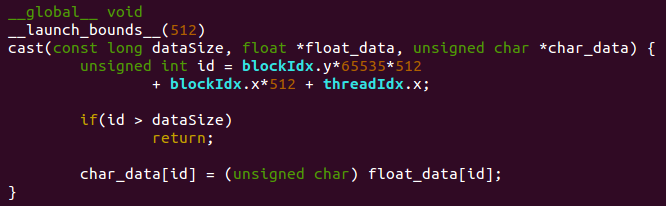
\includegraphics[width=3.5in]{simple_kernel}
\caption{A simple \texttt{CUDA} kernel example performing image data conversion from float to unsigned char.}
\label{kernel}
\end{figure}
	
\subsubsection{Our implementation}
Due to a lack of time on this project, neither signal filtering nor image filtering have been considered here even if such filtering is possible on modern GPUs. Image cropping was not necessary.

\textbf{Fig.\ref{kernel}} shows a simple kernel performing the data conversion operation. Note the \ac{simd} coding style : there are simultaneous parallel computations, but only a single instruction at a given moment. Lets say $N_i$ is the number of images we loaded at the first step. 
The $dataSize$ variable counts the total number of pixels ($dataSize=N_i\times L_x\times L_y$ assuming we did not crop anything) and the $id$ is a variable designating the current thread, starting at 0. Since the max $id$ can exceed the number of pixels $dataSize$, a simple if statement prevent the program to access prohibited memory. 

\subsection{Grid construction}

\subsubsection{Computing bounding box}

The third step in the reconstruction procedure is the establishment of coordinate system configuration for the reconstruction including its origin, its dimension and volume grid spacing. 
As our system has no need to predefine a volume before data acquisition we can use a simple bounding box technique as proposed by T. Wen \textit{et al.} \cite{2}.
A bounding box can be represented with two points only, $X_{min} = (x_{min},y_{min},z_{min})^T$ and $X_{max} = (x_{max}, y_{max}, z_{max})^T$ as showed in \textbf{figure \ref{bounding_box}}.

\begin{figure}[ht!]
\centering
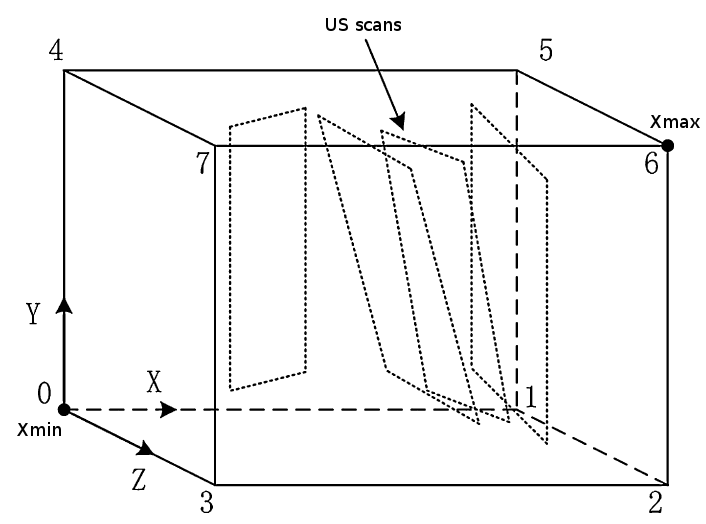
\includegraphics[width=3.2in]{bounding_box}
\caption{The resulting bounding box defined by $X_{min}$ and $X_{max}$. Image adapted and modified from T. Wen \textit{et al.} \cite{2}}
\label{bounding_box}
\end{figure}

With the notations of Eq.2 and Eq.3, the algorithm to find the bounding box is pretty straightforward :

\begin{samepage}
\begin{algorithm}
	\KwData{$X_{min} \gets (+\infty,+\infty, +\infty)$
		$X_{max} \gets (-\infty,-\infty, -\infty)$}
	\For{each image $I_i$}{
		\For{each of the four corner vertices $v_j$ of $I_i$}{
			$X_p^j \gets \text{image coordinate of } v_j$;
			$X_v^j \gets M_i\;M_{model}\;X_p^j$\;
			\If{point $X_v^j$ outside of the bounding box}{Update $X_{min}$ and $X_{max}$\;}
		}
	}
\caption{Bounding box algorithm}
\label{bbox_algo}
\end{algorithm}
\end{samepage}

\newpage
The test to know whether the point is in the bounding box or not consists of 6 scalar comparisons, and thus this algorithm can be executed safely on CPU without any performance drawbacks.
The origin of the volume is then placed at $X_{min}$.

At the end of this algorithm, all US images are contained in this bounding box and $X_{min}$ and $X_{max}$ are reached by one ultrasound image corner at least once.

The next step is to choose a voxel size. This is a critical parameter because the memory footprint of the grid is what hinders GPGPU volume reconstruction. 

\subsubsection{Choosing a voxel size}

Lets assume $W_b\times H_b\times L_b$ are the width, height and length of the generated bounding box, $W_g\times H_g\times L_g$ are the width, height and length of the grid (in voxels) and $\delta_v$ is the cubic voxel size. With those notations, we need to allocate at least a grid of $N_v = W_g\times H_g\times L_g =  \dfrac{W_b}{\delta_v}\times \dfrac{H_b}{\delta_v}\times \dfrac{L_b}{\delta_v}$ voxels. \par

\vspace{0.2cm}
Thus, memory cost is cubical with the number of subdivisions $N_s$. Each time we want to double precision, we have to pay eight times more memory.

\begin{table}[!hb]
\renewcommand{\arraystretch}{1.3}
\caption{Memory footprint for a $50\times 50\times 50$mm bounding box and unsigned char voxels}
\centering
\begin{tabular}{|c|c||c|c||c|}
\hline
$log_2(N_s)$ & $N_s$ & $\delta_v (\mu m)$ & $N_v$ & Grid memory \\
\hline
12 & 4096 & 12.2 & $2^{36}$ & 68.7GB\\\hline
11 & 2048 & 24.4 & $2^{33}$ & 8.59GB\\\hline
10 & 1024 & 48.8 & $2^{30}$ & 1.07GB\\\hline
9 & 512 & 97 & $2^{27}$ & 134MB\\\hline
8 & 256 & 195 & $2^{24}$ & 16.8MB\\\hline
7 & 128 & 390 & $2^{21}$ & 2.1MB\\\hline
\end{tabular}
\label{memory_table}
\end{table}
\textbf{Table \ref{memory_table}} shows grid memory consumption for a bounding box which is approximately the size of the bounding box obtained when scanning our intra-articular cartilage.
We see that when the voxel size $\delta_v$ goes under $100\mu m$ the memory begins to cause some problems to our GPU memory.
Even if some professional graphic cards can have up to 12GB of memory, a simple $\delta_v$ set to $50\mu m$ can cause trouble.
In fact, as it is explained later in this paper, even simple volume reconstruction algorithm will require at least three such grids in the bin-filling stage.

\begin{figure}[!ht]
\centering
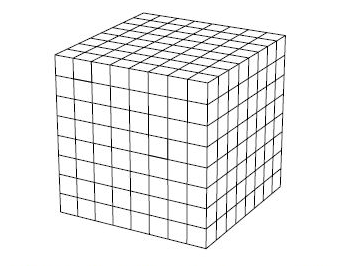
\includegraphics[width=2.5in]{grid}
\caption{A cubic bounding box split with $N_s=8$}
\label{grid}
\end{figure}

For example to perform an average in a \acl{simd} manner, we need at least two unsigned int grid and one unsigned char grids which almost multiply the \textbf{table \ref{memory_table}} grid memory footprint by 10 when assuming unsigned int are 4 bytes and unsigned char 1 byte.
That means that $\delta_v=0.05mm$ entails at least $10.70GB$ memory consumption just for the grids on the GPU memory.
Adding to that the size of the images, the system graphical environment load and the execution stack and our 12GB professional graphic card wont survive under such memory load.

The only solution is to split the grid into subgrids on the GPU side, and keep the whole voxel grid on the CPU side. The amount of splitting depends of the graphic card runtime available memory and the reconstruction algorithm used.

\subsubsection{Splitting the grid}
To ease grid splitting we round each grid side voxel size $W_g$, $H_g$, and $L_g$ to upper power of two to get a grid surrounding our bounding box :

\begin{eqnarray}
	W_G = 2^{\lceil log_2(W_g) \rceil}\\
	H_G = 2^{\lceil log_2(H_g) \rceil}\\
	L_G = 2^{\lceil log_2(L_g) \rceil}
\end{eqnarray}


This is far from being an optimal splitting method as a simple layer of voxel in each directions can enlarge the grid by a factor of 8 and thus multiply by 8 memory footprint and computation time. 
If execution time is still critical after having ported volume reconstruction algorithms to GPGPU, adapting the code to handle different grid sizes is worth the investment.

One of the greatest benefit of having computed the upper power of two grid is that we can divide the grid in power of two subgrids and all the subgrids will have the same dimension, simplifying the implementation. Moreover this could be used for further optimisation when using multiresolution grids to reduce global grid memory footprint. 

\begin{figure}[!ht]
\centering
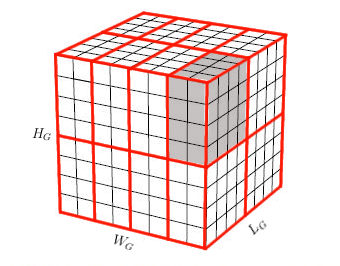
\includegraphics[width=2.5in]{subgrid}
\caption{The same cubic grid split in subgrids with $S_x = 4$, $S_y=2$ and $S_z=2$. One of the 16 subgrids is represented in grey.}
\label{subgrids}
\end{figure}

\textbf{Fig.\ref{subgrids}} shows the same grid as before. Because $W_g$, $H_g$ and $L_g$ were already powers of two, the upper power of two grid is the same. The grid is split with three parameters, $S_x$, $S_y$ and $S_z$ which represent the splitting amount along the x, y and z-axis (width, height, and length). Those parameters are powers of two. The resulting subgrid is like the original grid, a power of two grid. 
\begin{samepage}
The numbers of subgrids is given by the simple equation :
\begin{equation}
	N_{SG} = S_x\;S_y\;S_z
\end{equation}
\end{samepage}

\begin{samepage}
The size of those subgrids is given by :
\begin{eqnarray}
	W_{SG} = \dfrac{W_G}{S_x}\\
	H_{SG} = \dfrac{H_G}{S_y}\\
	L_{SG} = \dfrac{L_G}{S_z}
\end{eqnarray}
\end{samepage}

The grid is, like the images, stored in a contiguous array in the CPU memory. Accessing the voxel (i,j,k) is done by accessing the voxel at position $k\text{x}W_G\text{x}H_G + j\text{x}W_G + i$ in the array.
Because we want to keep data locality within the grid, we give splitting priority on the z-axis, the y-axis and finally the x-axis.

Once we have chosen a volume reconstruction algorithm, we know exactly how much space we will need for a given voxel size $\delta_v$. After fetching GPU available memory, we can compute a minimum grid splitting ratio $Sr$. As we can only divide by a power of two, we take the upper power of two of this ratio,  $S_R = 2^{\lceil log_2(S_r) \rceil}$.

\begin{samepage}
\begin{algorithm}
\KwData{The size of the grid $W_G=2^p$, $H_G=2^q$ and $L_G=2^r$\\
\hspace{1.15cm}The minimum upper power of two\\
\hspace{1.15cm}splitting ratio $S_R=2^s$}
\KwResult{The splitting ratio on each axis $S_x=2^i$, $S_y=2^j$ and $S_z=2^k$}
\vspace{0.5cm} $i\gets0;$ $j\gets0;$ $k\gets0;$\\
\While{$s>0$}{
	\eIf{$p \text{\textgreater} q \And p \text{\textgreater} r$}{
		$i\gets i+1$;\\
		$p\gets p-1$;
	}{
		\eIf{$q \text{\textgreater} r$}{
			$j\gets j+1$;\\
			$q\gets q-1$;
		}{
			$k\gets k+1$;\\
			$r\gets r-1$;
		}
	}
	$s\gets s-1$;\\
}
\caption{Splitting algorithm}
\label{split_algorithm}
\end{algorithm}
\end{samepage}

\subsubsection{Splitting algorithm}

\begin{figure*}[hb!]
\centering
\subfloat[VNN]{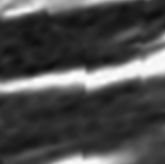
\includegraphics[width=1in]{VNN}%
\label{fig_first_case}}
\hfil
\subfloat[PNN]{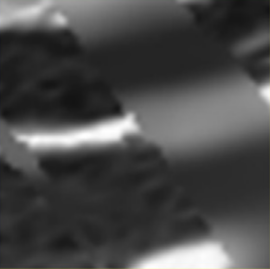
\includegraphics[width=1in]{PNN}%
\label{fig_first_case}}
\hfil
\subfloat[DW]{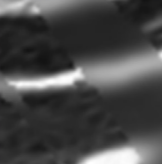
\includegraphics[width=1in]{DW}%
\label{fig_first_case}}
\hfil
\subfloat[FMM]{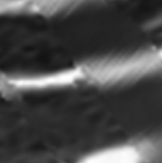
\includegraphics[width=1in]{FMM}%
\label{fig_first_case}}
\caption{Volume reconstruction methods comparison. Example of reconstructed slices extracted from \cite{2}.}
\label{algo_comparison}
\end{figure*}


After \textbf{algorithm \ref{split_algorithm}} we just need to allocate a grid of the size of one subgrid on the GPU and execute volume reconstruction algorithm on each of the subgrids one after another.

\section{Volume Filling}

Volume filling is the key procedure in the freehand 3D ultrasound systems \cite{3,4,6}. Various types of reconstruction algorithms have been reported and evaluated in \cite{10}. These algorithms can be grouped into three categories : \acl{vnn} (VNN), \acl{pnn} (PNN) and \acl{dw} (DW) interpolation algorithms. 
More elaborated algorithms methods are based on radial basis functions, such as spline interpolation functions \cite{11}, or statistical Bayesian model with Rayleigh distribution \cite{12}, but they are not suited for isotropic volume reconstruction (voxels).\par

\subsection{Existing algorithms}

VNN is the most intuitive method. It traverses each voxels, finds its nearest pixel by computing the shortest distance between the voxel and the sampled US images and inserts the nearest pixel value to the voxel \cite{13}.
Although this algorithms can preserve the most original texture, ultrasonic echo with speckle noise, it also trends to generate large artifacts when the minimum distance to pixel becomes large.\par

PNN interpolation method is the most popular reconstruction algorithm, which traverses on each pixel in the US images and assigns the pixel value to the nearest voxel.
The algorithm is done in two stages :
\begin{itemize}
	\item \textbf{Bin-filling:} In the bin-filling stage each pixel is traversed and its pixel value is assigned to its nearest voxel. For a given voxel, multiple pixel contributions are generally handled by averaging pixel intensities.  
	\item \textbf{Hole-filling:} In the hole-filling stage, the algorithm traverses on each voxel and fills each empty voxels by local neighborhood averaging. Most hole filling algorithms depend on the interpolation gaps, and there can still be few holes if the distance among sampled US images is to far apart, greater than the interpolation radius. 
\end{itemize}
With the PNN method, obvious artefacts can observed on the boundaries between the highly detailed bin-filled regions and the smoothed hole-filling regions.\par

Similar to the VNN interpolation method, DW interpolation proceeds voxel by voxel but instead of using the nearest pixel, each voxel value is assigned with a weighted average of pixel situated nearby. The parameters to choose are the weighting function, and the size and shape of the neighborhood. The simplest approach employs a spherical neighborhood. All the pixels in the sphere are weighted by the inverse distance to the voxel and are then averaged. If the radius is too large, the reconstructed volume will be highly smoothed.

For the interpolation stage (hole-filling), we can use the Fast Marching Method (FMM), proposed by T. Wen \textit{et al.}\cite{2}. The proposed marching process ensures that the direction of information propagation is the normal direction of the evolving boundary, improving edge preservation in the hole-filled areas.
\textbf{Fig.\ref{algo_comparison}} shows an example of reconstructed slice generated by those algorithms.

According to T. Wen \textit{et al.}\cite{2} typical execution time for a $421\times425\times131$ grid and 138 images is 8849s for VNN, 94s for PNN, 15523s for DW, and 134s for FMM.
We observe that it is highly time demanding for the VNN and conventional DW interpolation algorithm to find the shortest distance for each voxel among hundreds of sampled US images. Several hours are needed to complete the reconstruction. Such expensive computation time is usually unbearable in most clinical applications. In our case, the grid is approximately 1 to 10 times bigger, and we have 10 to 20 times more images. Thus, only PNN and FMM are good candidates for further GPGPU optimisations.

\section{Adapting PNN to CUDA}

PNN was the simplest algorithm and thus was chosen in first place. 
In the bin-filling stage each pixel is traversed and its pixel value is assigned to its nearest voxel. 
For a given voxel, multiple pixel contributions are handled by averaging pixel intensities.  
In the hole-filling stage, the algorithm traverses on each voxel and fills each empty voxels by local neighborhood averaging. The pattern chosen here is a sphere with $R_k$ interpolation radius (in voxels). 


\begin{figure}[ht!]
\centering
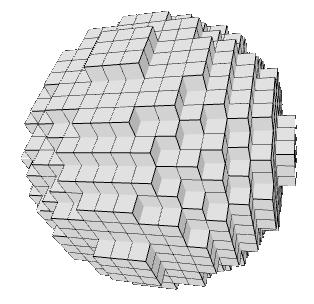
\includegraphics[width=2.5in]{neighborhood}
\caption{A spherical voxel neighborhood with $R_k=9$.}
\label{neighborhood}
\end{figure}

\subsubsection{Quick introduction to \texttt{CUDA}}
In \texttt{CUDA}, the CPU is called \textbf{host} and the GPUs are called \textbf{devices}. 
Each of these devices can execute functions that are written in a SIMD manner, called \textbf{kernels}. 
A kernel is executed by an array of \textbf{threads}, all threads run the same code at the same time, and each thread has an ID that it uses to compute memory addresses and make control decisions. 
Kernel launches a grid of \textbf{thread blocks}, threads within a same block can cooperate and synchronize, and threads in different blocks cannot. 
Each device is free to schedule thread blocks on any multiprocessor but only one kernel can execute on a device at one time.
All kernel launches are asynchronous, control returns to host (CPU) immediately and kernel executes after all previous \texttt{CUDA} calls have completed.
Synchronization with devices can be forced by calling the special \texttt{CUDA} function $cudaThreadSynchronize()$ which blocks the execution flow until all previous \texttt{CUDA} calls complete.
Synchronization within a thread block is achieved through another function, \_\_$syncthreads()$ and generates a barrier synchronization instruction, no thread can pass this barrier until all threads in the block reach it.
This function is only allowed in conditional code if the conditional is uniform across the entire thread block or it will result in a deadlock.
\texttt{CUDA} provides some \textbf{atomic functions}, 32-bit words atomic operations in global memory for compute capability 1.1 and higher, and 32 and 64-bit words for compute capability 1.2 and higher, including associative operations like addition, increment, maximum, logical bitwise operations, exchange and compare and swap (CAS).
Global memory is large (usually 512MB to 2GB), has high latency and is not cached, but it is accessible by all threads.
Shared memory is stored in on-chip shared memory which has very low latency and is accessible by all threads in the same thread block.
It has the lifetime of a thread block.
Scalars and built-in vector types are stored in registers. What does not fit in registers spills to local memory.

The main problem when adapting an algorithm to GPGPU is memory and thread concurrency. 

\subsection{Device memory management}

\begin{figure*}[!ht]
\centering
\subfloat{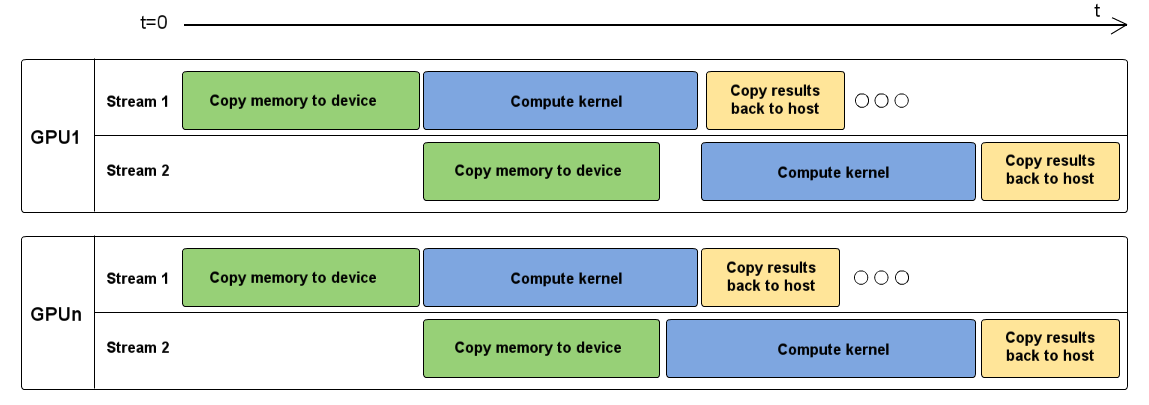
\includegraphics[width=7in]{basic_streams}%
\label{fig_third_case}}
\caption{Example of two streams concurrent execution. Kernel execution and memory transfers are done simultaneously on different streams. On $GPU_n$, two kernels are executing in parallel on the same device.}
\label{basic_streams}
\end{figure*}


We already solved the problem of the GPU memory size by splitting the grid into subgrids by a certain ratio, but doing so raises other problems.
Memory transfers are expensive, especially when the kernel workload is low.
In fact, transfers between the host and device are the slowest link of data movement involved in GPU computing.
Sending data from host to device or from device to host is limited by the memory link (8GB/s on PCIe x16 Gen2) and the GPU memory clock rate (usually 6GB/s peak bandwidth on regular Nvidia GPUs).
Higher bandwidth is achieved between the host and the device only when using large chunk of pinned (page-locked) memory.
The thing you need to know is that data transfers between the host and device can sometimes be overlapped with kernel execution and other data transfers.
This can be done by using \texttt{CUDA} \textbf{streams}.\par
A stream is a sequence of operations that execute in issue-order on the GPU.
It allows to go beyond multi-threaded parallelism, giving the ability to perform multiple \texttt{CUDA} operations simultaneously (kernels and memory transfers).
For example, the Fermi architecture (compute capability 2.0+) can simultaneously support up to 16 \texttt{CUDA} kernels per GPU, 2 memory transfers (one to the device and one to the host) and computations on the CPU.
\texttt{CUDA} operations in different streams may run concurrently, and may be interleaved. \textbf{Fig.\ref{basic_streams}} shows an example of concurrent device execution on two streams.

\subsection{Bin-filling}
In order to compute an average on a \ac{simd} architecture, we need at least an array to sum the pixel contributions for each voxel and an array counting the per voxel pixel contributions.
We call these arrays the \textbf{mean subgrid} and the \textbf{hit subgrid}.
If we want to apply our stream strategy, we need an additional array which stores the last computed result.
We simply name it the \textbf{voxel subgrid}. 
In addition to these arrays, we need memory for the images and transformations.
\textbf{Fig.\ref{bin_filling_memory}} shows memory blocks on host and device $GPU_i$.
\vspace{0.5cm}
\begin{figure}[hb!]
\centering
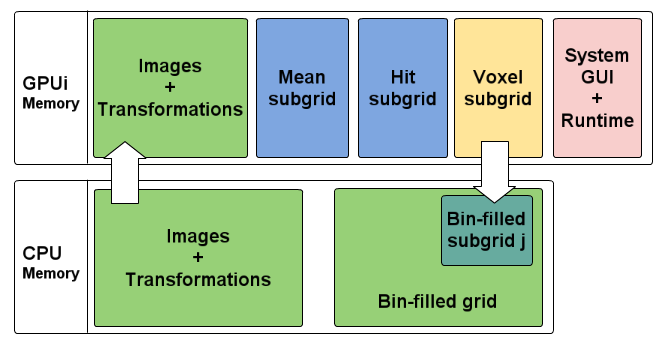
\includegraphics[width=3.5in]{bin_filling_memory}
\caption{Memory layout for the PNN bin-filling. Memory transfers are represented with white arrows.}
\label{bin_filling_memory}
\end{figure}

\begin{algorithm}
\KwData{Thread Id, grid and subgrid size, subgrid Id, voxel size, images, transformations, target hit and mean subgrid.}
\KwResult{Updated hit and mean subgrid.}
\vspace{0.2cm}
Compute current pixel image position;\\
\If{Pixel position out of range}{return;}
Apply transformation to current pixel;\\
Compute voxel position in grid;\\
\If{Current voxel not in current subgrid}{return;}
Compute voxel position in subgrid;\\
Atomically increment current voxel hit subgrid;\\
Atomically add current voxel intensity to mean subgrid;\\
\caption{Bin-filling kernel (step 1).}
\label{bin_filling_kernel}
\end{algorithm}

\newpage
\textbf{Appendix A} shows the whole host side volume reconstruction process, including memory allocations and memory transfers. 
\textbf{Algorithm \ref{bin_filling_kernel} and \ref{compute_mean_kernel}} shows the bin-filling \texttt{CUDA} implementation.

We use one thread per pixel with $32\times 32$ thread-blocks.
That means that our images are processed in $32\times 32$ blocks on each multiprocessor, executing 1024 threads at once.
Memory transactions are close to optimal as each warp (32 threads) will request 32 bytes (32 unsigned pixel values) of contiguous memory aligned on a 32 byte address, each representing a line of our 32x32 sub-image.
We can get four times more performance for images memory transactions by processing 4 pixels per thread and fetching 128 bytes (32 integers, 4 pixels per integer) representing 64x64 sub-images at once, maximizing device memory throughput.
Because images are $64\times 1296$ and $1296 \mod{32} = 16$, we need to check whether the current pixel array position is not out of bound in the kernel.


Accessing forbidden memory results in undefined behaviours on the device, and can corrupt data or crash the kernel.
An interesting tool to detect such bad accesses is \textit{cuda-memcheck} and \textit{cuda-gdb}.
Another interesting tool is the Nvidia Visual Profiler \textit{nvvp}, which allows to visualize the execution of streams on multiple devices.\par
After having computed pixel and voxel positions, we need to check whether the current voxel where the pixel would contribute is in the current computed subgrid. 
If so, because multiple threads can write to the same voxel location at the same time, hit and mean grid modifications must be done atomically.\par
Finally, another dedicated kernel (\textbf{algorithm \ref{compute_mean_kernel}}) computes the real mean, by dividing the mean subgrid by the hit subgrid and storing the result in the voxel subgrid which is then moved back to the host.


\begin{algorithm}
\KwData{Thread Id, source hit and mean subgrid, target voxel subgrid.}
\KwResult{Updated voxel subgrid.}
\vspace{0.2cm}
Compute current voxel position in subgrid;\\
\If{Voxel position out of range}{return;}
\eIf{Current voxel hit grid value == 0}%
{$\text{Target voxel intensity }\gets 0$;}%
{$\text{Target voxel intensity }\gets \text{mean intensity value}$;}

\caption{Bin-filling kernel (step 2), computing mean.}
\label{compute_mean_kernel}
\end{algorithm}

\begin{figure*}
\centering
\subfloat[Exaggerated grid splitting of a single reconstructed slice]{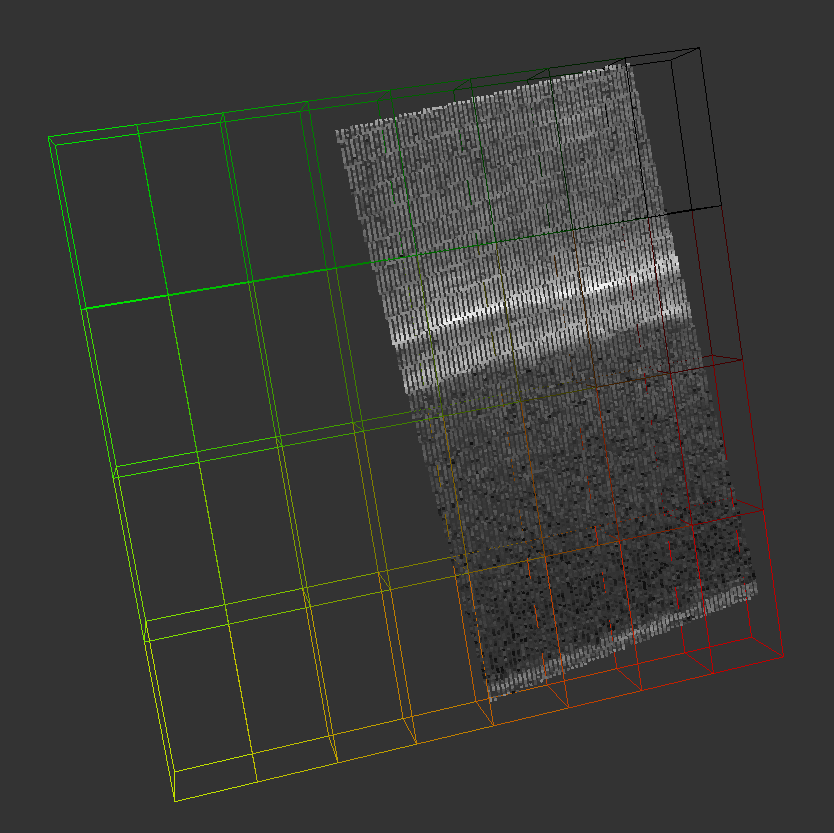
\includegraphics[width=2.75in]{split1}}%
\label{mega_grid_splitting}
\hfill
\subfloat[An extracted 2D slice from reconstructed 3D volume after the bin-filling stage.]{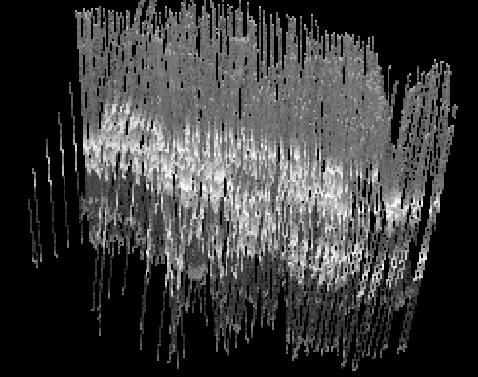
\includegraphics[width=3.0in]{pnn_slice}}%
\label{extracted_pnn_slice}
\hfill
\subfloat[Reconstructed volume in its grid. Note the memory waste when taking the surrounding power of two voxel grid.]{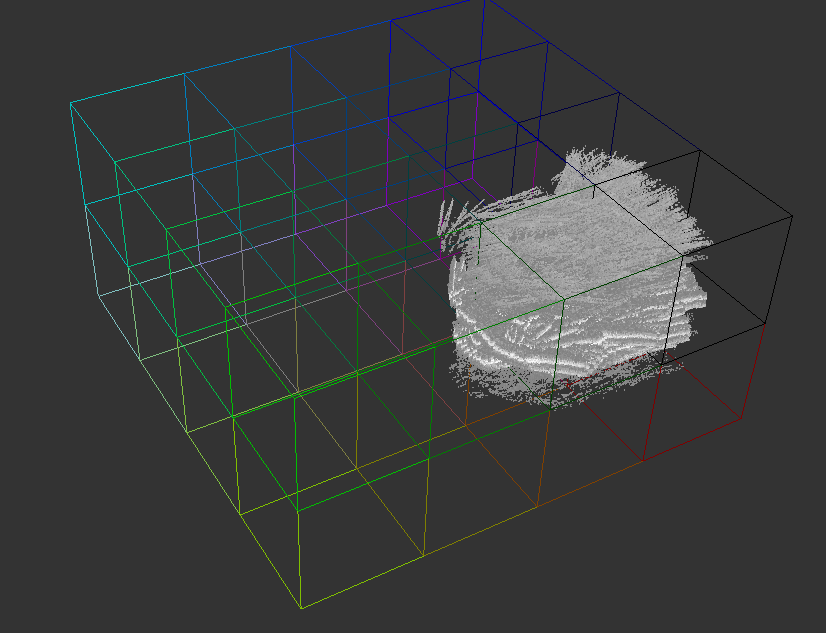
\includegraphics[width=3.0in]{split2}}
\label{reconstructed_pnn_volume2}
\hfill
\subfloat[Top view of the same reconstructed volume as (c).]{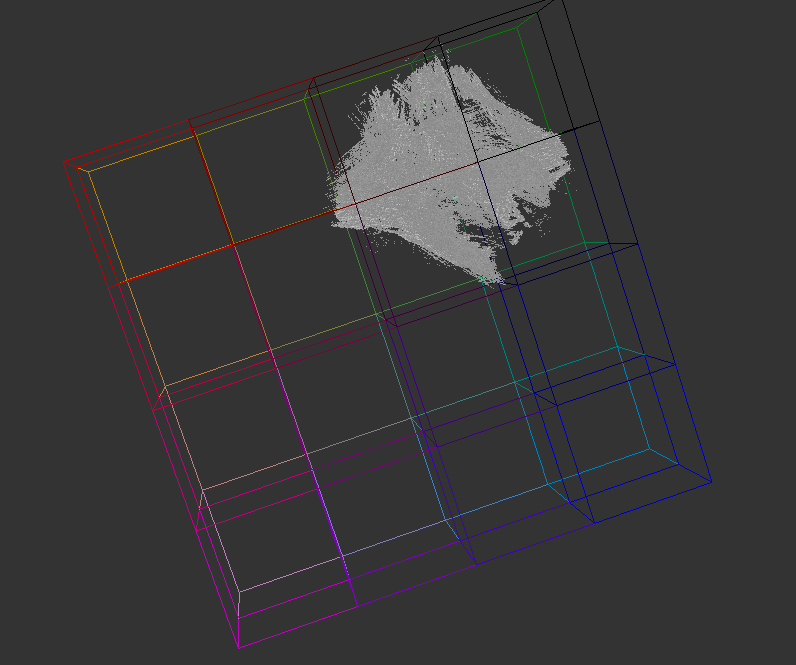
\includegraphics[width=3.0in]{bad_grid}}
\label{bad_grid}
\hfill
\subfloat[Reconstructed 3D isotropic volume. No position filtering.]{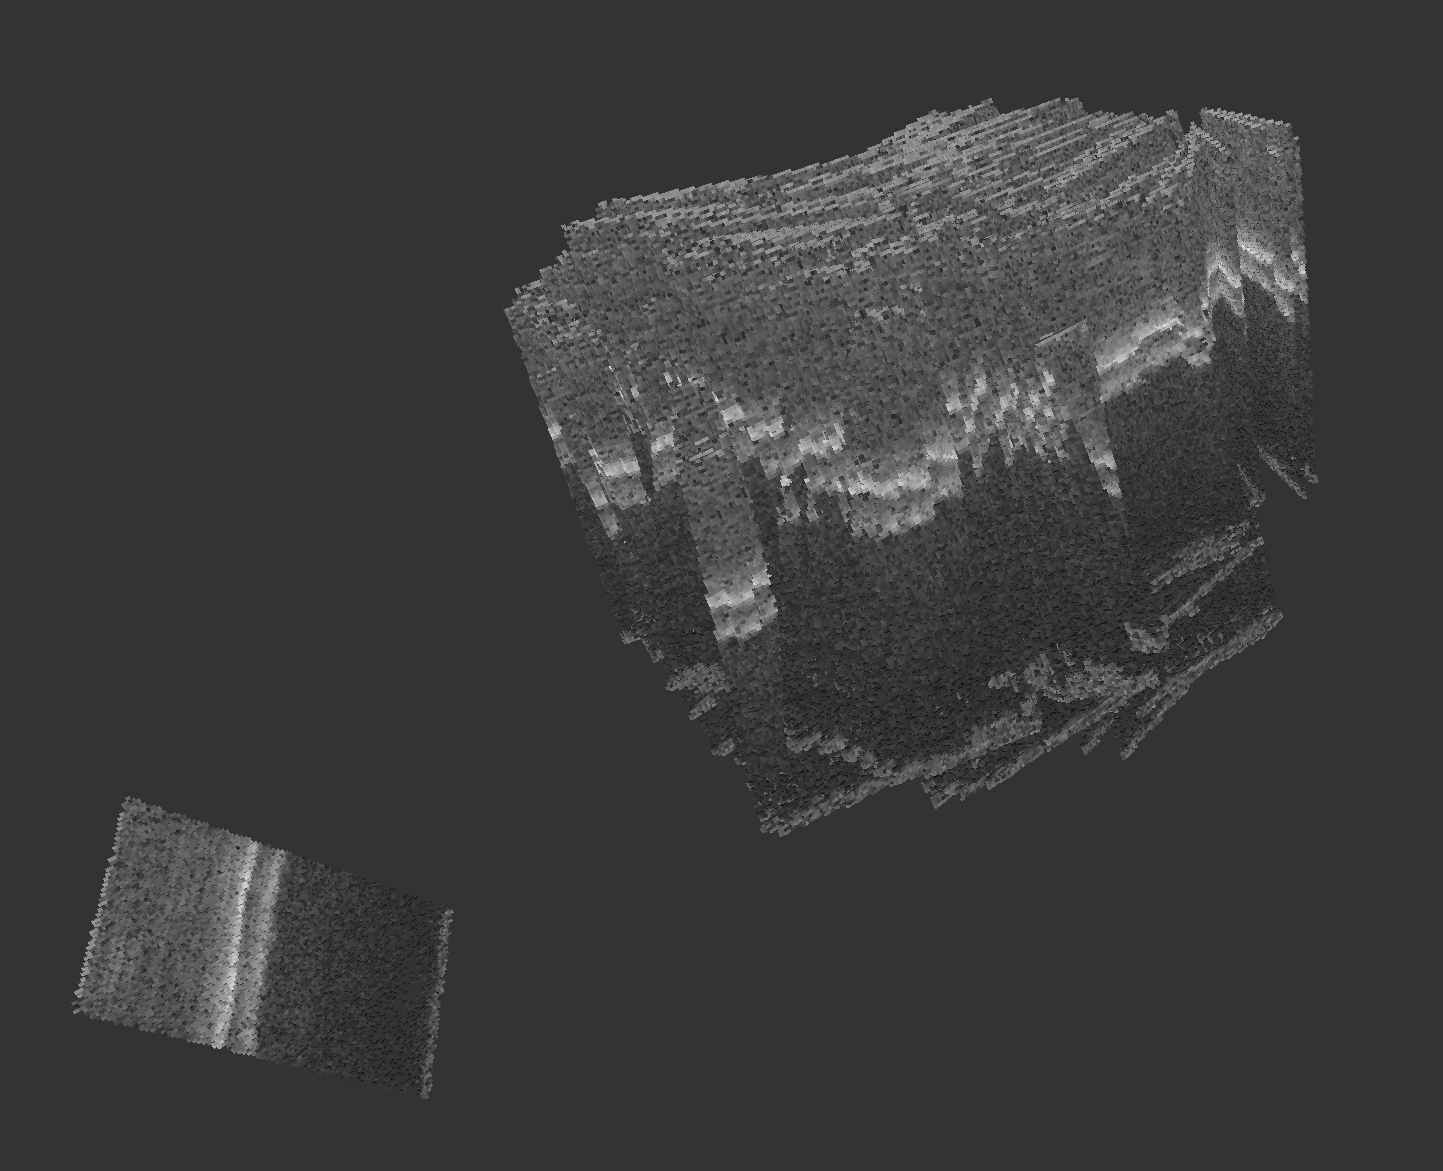
\includegraphics[width=3.0in]{data_1}}
\label{reconstructed_pnn_volume}
\hfill
\subfloat[Thresholded volume. The white voxels represent the cartilage interface.]{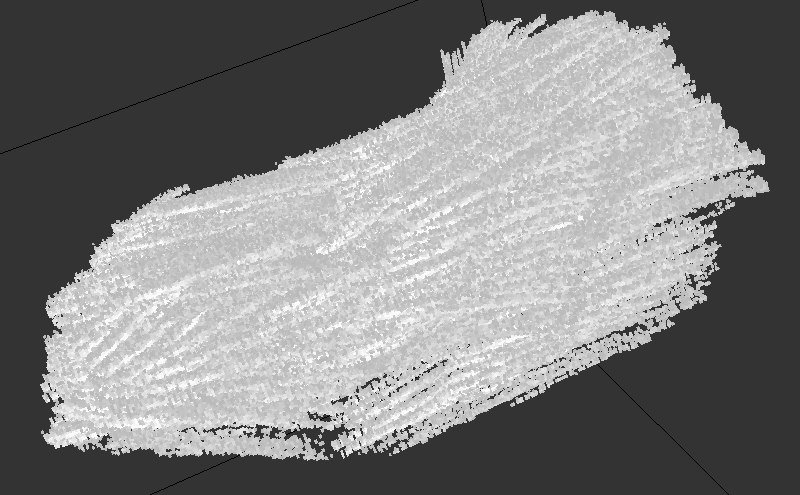
\includegraphics[width=3.0in]{results1}}
\label{cartilage_volume}
\hfill
\caption{Results after bin-filling stage}
\label{pnn_image_group}
\end{figure*}


If the hit subgrid voxel value is 0, that means that the voxel is a hole and the resulting value is in voxel subgrid is set to 0.
This kernel can only be executed when the last memory transfer to the host has finished, but during bin-filling kernel computation, the other stream might already have finished to copy back the last voxel subgrid to the host.\par
\textbf{Fig.\ref{pnn_image_group}a} shows a single reconstructed slice after the bin-filling stage. \textbf{Fig.\ref{pnn_image_group}b} shows a extracted 2D slice of a reconstructed volume from multiple images after bin-filling. \textbf{Fig.\ref{pnn_image_group}e} shows the source bin-filled volume.

\subsection{Hole-filling}

In order to compute hole-filling, we need a source subgrid, the \textbf{hole-filled subgrid}, and a destination subgrid, the \textbf{bin-filled subgrid}. \textbf{Fig.\ref{hole_filling_memory}} shows the new memory layout.

\begin{figure}[ht!]
\centering
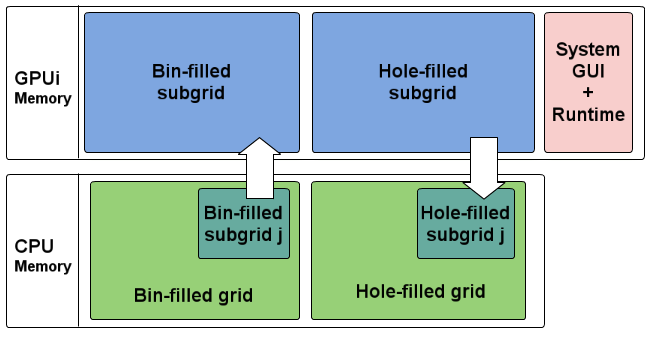
\includegraphics[width=3.0in]{hole_filling_memory}
\caption{Memory layout for the PNN hole-filling. Memory transfers are represented with white arrows.}
\label{hole_filling_memory}
\end{figure}
 

Because we do not need image data and three grids of various size anymore, we gained much space on the device memory. Thus we can resplit the whole host grid in bigger subgrids to improve hole filling performance. The chosen thread blocks are 1024 consecutive voxels, resulting in one thread per subgrid voxel.
As we are using local neighborhood averaging in a spherical shape, the implementation of hole filling is pretty straightforward. \textbf{Algorithm \ref{hole_filling_algorithm}} shows a simple hole-filling kernel.


\begin{algorithm}
\KwData{Thread Id, $R_k$, source bin-filled subgrid and destination hole-filled subgrid.}
\KwResult{Updated hole-filled subgrid.}
\vspace{0.2cm}
Compute current voxel position in subgrid;\\
\If{voxel is not a hole}{return;}
\If{voxel to close to one subgrid border}{%
\textcolor{OliveGreen}{//This will be handled on host side}\\
return;}
$k\gets0$; $s\gets0$;\\
\For{each voxel $i$ in spherical neighborhood of radius $R_k$}%
{\If{voxel $i$ is not a hole}%
{$s\gets s + \text{voxel }i\text{ intensity}$;\\
$k\gets k + 1$;}}
\eIf{$k == 0$}{Hole filled voxel value $\gets 0$;}{Hole filled voxel value $\gets s/k$}

\caption{Simple hole-filling kernel.}
\label{hole_filling_algorithm}
\end{algorithm}

The problem when splitting the grid is that we can not reconstruct the voxel located near the borders of the subgrid because neighborhood information is lost. One solution is to send a slightly bigger subgrid to the device which includes this information. Another much simpler solution is to compute hole-filling in such area directly on the host CPU, during the execution of the kernels. The kernels will still be in charge of most of the subgrid inner volume, which is where the heavy workload is.

To improve this hole-filling we can take advantage of shared memory.
Here each voxel will try to access to all its neighbors within a given range and these memory accesses are strided resulting in too many memory transactions.
A simple way to fix this is to copy the per warp (32 voxels) neighborhood in the shared memory so that the high latency expensive global memory accesses are done just once and following accesses are done on the much faster cached local memory (roughly 100 times faster).
But due to its small size (usually $64kB$ per multiprocessor) it is not always possible to store the whole thread block voxel neighborhood in shared memory, especially when the radius $R_k$ is large.
For such case we can attach a 3D texture to the bin-filled source subgrid.
Cuda texture are read-only and memory space is cached.
Therefore, a texture fetch costs one device memory read only on a cache miss, otherwise, it just costs one read from the texture cache.
The texture cache is optimized for 2D or 3D spatial locality, so threads of the same warp that read texture addresses that are close together will achieve best performance and that is exactly our scenario.

\subsection{Results}

The whole volume reconstruction process has been developed in \texttt{C++}.
For the \texttt{CUDA} part, we used the \texttt{CUDA} Toolkit 5.5.
A basic Graphical User Interface (GUI) has been developed to visualize the reconstructed volume with different thresholds and to easily generate 2D slices.
This GUI was made with $Qt4$ and the $QGLviewer$, and the voxel renderer was done with $OpenGL$ with the help of $\texttt{CUDA}$ for the heavy computations (millions of voxels).

\textbf{Fig.\ref{pnn_image_group}c and \ref{pnn_image_group}d} shows a reconstructed isotropic volume. \textbf{Fig.\ref{pnn_image_group}f} shows the cartilage interface.

\subsubsection{Execution times}

\begin{table*}[!ht]
\renewcommand{\arraystretch}{1.3}
\caption{Executions times on a GTX590 (dual GPU card) with $2\times1.5$GB embed memory and 8GB CPU memory}
\label{results_gtx590}
\centering
\begin{tabular}{|c|c|c||c|c||c|c|c|c||c|}
\hline
$W_G$ & $H_G$ & $L_H$ & $\delta_v$ & $N_{SG}$ & Data Loading & Bounding Box & Bin-Filling & Hole-Filling & Total \\
      &&&$(\mu m)$&&(ms)&(ms)&(ms)&(ms)&(ms)\\
\hline
\multicolumn{10}{|l|}{\textbf{Dataset 1 :} Single US image}\\
\hline
64&32&8&500&-&-&-&-&-&-\\
\hline
128&128&16&200&-&-&-&-&-&-\\
\hline
256&256&32&100&-&-&-&-&-&-\\
\hline
\hline
\multicolumn{10}{|l|}{\textbf{Dataset 2 :} Half tibia plateau (1610 images)}\\
\hline
128&256&128&500&-&-&-&-&-&-\\
\hline
256&512&512&200&-&-&-&-&-&-\\
\hline
512&1024&1024&100&-&-&-&-&-&-\\
\hline
\hline
\multicolumn{10}{|l|}{\textbf{Dataset 3 :} Full femur neck (3770 images)}\\
\hline
256&128&256&500&-&-&-&-&-&-\\
\hline
1024&512&1024&200&-&-&-&-&-&-\\
\hline
2048&1024&2048&100&-&-&-&-&-&-\\
\hline
\end{tabular}
\end{table*}

\begin{table*}[!ht]
\renewcommand{\arraystretch}{1.3}
\caption{Executions times on two GTX670 with 4GB embed memory each and 16GB CPU memory}
\label{results_gtx670}
\centering
\begin{tabular}{|c|c|c||c|c||c|c|c|c||c|}
\hline
$W_G$ & $H_G$ & $L_H$ & $\delta_v$ & $N_{SG}$ & Data Loading & Bounding Box & Bin-Filling & Hole-Filling & Total \\
      &&&$(\mu m)$&&(ms)&(ms)&(ms)&(ms)&(ms)\\
\hline
\multicolumn{10}{|l|}{\textbf{Dataset 1 :} Single US image}\\
\hline
64&32&8&500&1&0&0&0&-&-\\
\hline
128&128&16&200&1&0&0&0&-&-\\
\hline
256&256&32&100&1&0&0&0&-&-\\
\hline
\hline
\multicolumn{10}{|l|}{\textbf{Dataset 2 :} Half tibia plateau (1610 images)}\\
\hline
128&256&128&500&1&290&0&70&-&-\\
\hline
256&512&512&200&1&280&0&100&-&-\\
\hline
512&1024&1024&100&1&270&0&180&-&-\\
\hline
\hline
\multicolumn{10}{|l|}{\textbf{Dataset 3 :} Full femur neck (3770 images)}\\
\hline
256&128&256&500&1&680&0&140&-&-\\
\hline
1024&512&1024&200&1&680&0&260&-&-\\
\hline
2048&1024&2048&100&8&680&0&480&-&-\\
\hline
\end{tabular}
\end{table*}

\textbf{Table \ref{results_gtx590}} and \textbf{table \ref{results_gtx670}} show typical execution times for various datasets on two different computers.
\textbf{The hole-filling step has not been implemented yet.} The bin-filling step is done in less than 1 second, even for massive data amount (3770 images and 2048x1024x2048 voxel grid).

\newpage
\section{Conclusion}
In this paper, we showed that reconstructing a isotropic volume from 2D localized ultrasound images was possible on GPU.
This was done by adapting an existing volume reconstruction algorithm knows as Pixel Nearest Neighbor (PNN) and using the massive parallelism provided by our every day GPUs.
This method offers huge speedup to volume reconstruction, even when not fully optimized, allowing to reduce drastically reconstruction time that would be otherwise unbearable for such clinical applications.
Nearly all desktop computers and professional laptops include a dedicated Graphic Processing Unit, which means that all this speedup comes for free, and that there is no extra cost.
However, PNN is not the best algorithm for such isotropic volume reconstruction. Adapting the Fast Marching Method proposed by T. Wen \textit{et al.} \cite{2} to \texttt{CUDA} is the next step to get rapid and more precise volume reconstruction.


\section*{Acknowledgments}
I would like to thank the TIMC-IMAG laboratory for having hosted me for 4 months, especially the GMCAO team members that were always here to help when there were any problems and for the good mood. Special thanks goes to M. Chabanas for having taken the time and energy throughout the project by providing precious feedbacks and for having introduced me to the TIMC-IMAG laboratory.

\appendices

\section{Adapted PNN algorithm pseudo code}

\begin{algorithm}
\KwData{The SoA filtered transformations and the cropped, smoothed and converted images.}
\KwResult{The reconstructed 3D isotropic volume}

\textcolor{OliveGreen}{//Bounding box and grid creation}\\
Compute bounding box with algorithm \ref{bbox_algo};\\
Choose voxel size $\delta_v$ and compute original grid size;\\
Compute upper power of two grid size with (5),(6) and (7);\\
Allocate new grid on host in pinned memory;\\

\textcolor{OliveGreen}{//Split grid}\\
\For{each GPU $i$ available}{
	Create two streams $s_1^i$ and $s_2^i$;\\
	Fetch available device memory $m_i$;\\
	Compute min grid split ratio $r_i$ with $m_i$;\\
}
Split grid with $max(r_i)$ with algorithm \ref{split_algorithm};\\

\textcolor{OliveGreen}{//Allocate data and send initial data to devices}\\
\For{each GPU i}{
	Allocate voxel, mean and hit subgrid on device $i$;\\
	Allocate image array and transformation arrays on device $i$;\\
	Send images and transformations from host to device $i$ on stream $s_1^i$;\\
}
Free CPU image and transformation data;
\textcolor{Blue}{Synchronize devices with host;}

\end{algorithm}
\begin{algorithm}
\textcolor{OliveGreen}{//Compute hole-filling}\\
$i \gets 0$;$j\gets 0$;\\
$N_{gpu}\gets \text{number of GPUs}$;\\
\For{each subgrid}{
	Compute bin-filling kernel 1 on device $i$ on stream $s_i^{j\mod{2}}$;\\
	Add memory transfer barrier on stream $s_i^{j\mod{2}}$;\\
	Compute bin-filling kernel 2 on device $i$ on stream $s_i^{j\mod{2}}$;\\
	Copy back computed subgrid to host from device $i$ on stream $s_i^{j\mod{2}}$;\\
	$i \gets (i+1)\mod{N_{gpu}}$;\\
	$j \gets j+1$;\\
}
\textcolor{Blue}{Synchronize devices with host;}\\
\textcolor{OliveGreen}{//Free memory and resplit grid}\\
\For{each GPU $i$}{
	Free grids, image and transformations arrays on device $i$;\\
	Fetch available device memory $m_i$';\\
	Compute new min grid split ratio $r_i$' with $m_i$';\\
}
Split grid with $max(r_i)$;\\

with algorithm \ref{split_algorithm}\\
\For{each GPU $i$}{
	Allocate 2 voxel subgrids;\\
}
\textcolor{OliveGreen}{//Compute bin-filling}\\
$i \gets 0$;$j\gets 0$;\\
\For{each subgrid}{
	Copy to device $i$ the bin-filled subgrid $j$ on stream $s_i^{j\mod{2}}$;\\
	Compute hole-filling kernel on device $i$ on stream $s_i^{j\mod{2}}$;\\
	Copy back hole-filled subgrid $j$ to host from device $i$ on stream $s_i^{j\mod{2}}$;\\
	$i \gets (i+1)\mod{N_{gpu}}$;\\
	$j \gets j+1$;\\
}
\For{each subgrid edge}{
	Compute hole-filling on CPU;
}
\textcolor{Blue}{Synchronize devices with host;}\\
\textcolor{OliveGreen}{//Display 2D slices, 3D voxel grid or do further processing}\\

\caption{Reconstruction algorithm pseudo code}
\label{reconstruction_algorithm}
\end{algorithm}

\bibliographystyle{IEEEtran}
\bibliography{master}

\end{document}


